\icode{N24W-MP-SI-L2-261004-005}
\nceeID[4]{2024安徽}{1}
大连相干光源是我国第一台高增益自由电子激光用户装置，其激光辐射所应用的玻尔原子理论很好地解释了氢原子的光谱特征。图为氢原子的能级示意图，已知紫外光的光子能量大于\qty{3.11}{eV}，当大量处于\(n = 3\)能级的氢原子向低能级跃迁时，辐射不同频率的紫外光有\paren[]

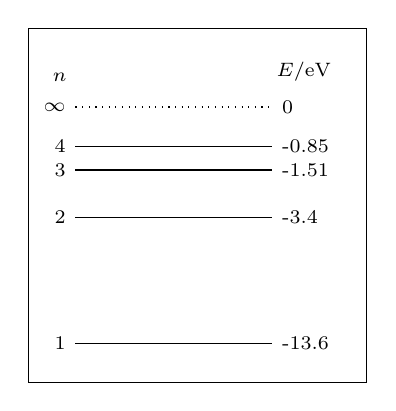
\begin{tikzpicture}[font=\scriptsize]
	\foreach \y/\n/\e in {0/1/-13.6,1.6/2/-3.4,2.2/3/-1.51,2.5/4/-0.85}
		\draw (0,\y)node[left]{\n}--(2.5,\y)node[right]{\e};
	\draw[dotted] (0,3)node[left]{\(\infty\)}--(2.5,3)node[right]{ 0};
	\node at(-.2,3.2)[above]{\(n\)};
	\node at(2.9,3.2)[above]{\(E\)/\qty{}{eV}};
	\draw (-.6,-.5) rectangle(3.7,4);
\end{tikzpicture}
\begin{choices}
	\item 1种
	\item 2种
	\item 3种
	\item 4种
\end{choices}
\begin{answer}
	B\qquad 提示：\(n = 3\) 至\(n = 1\) 、\(n = 2\) 至\(n = 1\)两种
\end{answer}